\chapter{Abordagem meta-heurística para o TSP}
\thispagestyle{empty}

Uma meta-heurística é um método heurístico para resolver problemas de otimização combinatória de forma genérica. Uma única meta-heurística pode ser reutilizada para resolver vários problemas diferentes, exigindo, por vezes, pouco esforço de adaptação para cada um deles. Este capítulo descreve a meta-heurística \textit{Iterated Local Search} (ILS), além das devidas adaptações necessárias para utilizá-la para resolver o TSP.

\section{\textit{Framework} ILS}
Considere um problema de otimização combinatória qualquer. Assuma que o problema é de minimização. O código a seguir apresenta um algoritmo genérico para resolvê-lo: 

%\begin{lstlisting}[style=cplusplusListStyle, caption={Framework do ILS.}, label={lst:ilsAlg}]
\begin{lstlisting}[style=cplusplusListStyle]
Solution ILS(int maxIter, int maxIterIls)
{
	Solution bestOfAll;
	bestOfAll.cost = INFINITY;
	for(int i = 0; i < maxIter; i++)
	{
		Solution s = Construcao();
		Solution best = s;
	
		int iterIls = 0;
	
		while(iterIls <= maxIterIls)
		{
			BuscaLocal(&s);
			if(s.cost < best.cost)
			{
				best = s;
				iterIls = 0;		
			}
			s = Perturbacao(best);
			iterIls++;
		}
		if (best.cost < bestOfAll.cost)
			bestOfAll = best;	
	}

return bestOfAll;
}
\end{lstlisting}

Primeiramente, algoritmo constrói uma solução baseando-se em palpites educados através do método Construção() (linha 7). Em seguida, tenta-se melhorar o custo dessa solução fazendo-se pequenas modificações através do método BuscaLocal() enquanto houver melhoras (linhas 14--18). Quando não for mais possível melhorar a solução, continua-se a partir de uma cópia levemente modificada da melhor solução da iteração corrente \texttt{best}, gerada pelo procedimento Perturbação() (linha 20). Continua-se até que um critério de parada seja atingido (linha 12). Se \texttt{best.cost} for menor que \texttt{bestOfAll.cost}, \texttt{best} passa a ser a melhor solução (linhas 23 e 24). Esse processo é repetido \texttt{maxIter} vezes (linha 5), e a melhor solução \texttt{bestOfAll} é retornada (linha 27).

Os procedimentos Construção(), BuscaLocal() e Perturbação() serão explicados em detalhes para o caso do TSP nas próximas seções. Recomenda-se que o leitor implemente-os na ordem em que são apresentados, para que então possa implementar o código acima.

\iffalse

O algoritmo possui três rotinas principais: (i) construir uma solução para a instância do problema baseando-se em palpites educados (método Construção()); (ii) buscar soluções parecidas com a solução corrente de forma a diminuir o seu valor objetivo através de pequenas modificações (método BuscaLocal()); e (iii) quando não for mais possível encontrar melhorias durante a busca local, modificar levemente a solução de forma aleatória (método Perturbação()).

\begin{figure}
    \begin{center}
    \scalebox{0.9}{
\begin{tikzpicture}[node distance=2cm, cross/.style={path picture={ 
  \draw[black]
(path picture bounding box.south east) -- (path picture bounding box.north west) (path picture bounding box.south west) -- (path picture bounding box.north east);
}}]
\tikzstyle{startstop} = [rectangle, rounded corners, minimum width=3cm, minimum height=1cm,text centered, draw=black, fill=red!30]
\tikzstyle{io} = [trapezium, trapezium left angle=70, trapezium right angle=110, minimum width=3cm, minimum height=1cm, text centered, align=center, draw=black, fill=blue!30]
\tikzstyle{process} = [rectangle, minimum width=3cm, minimum height=1cm, text centered, align = center, draw=black, fill=orange!30]
\tikzstyle{decision} = [diamond,aspect=2, minimum width=3cm, minimum height=1cm, text centered, align = center, draw=black, fill=green!30]
\tikzstyle{arrow} = [thick,->,>=latex, rounded corners]


\node (construction) [process] { \(s \leftarrow \text{Construção}()\)\\ \(s' \leftarrow s\) \\ \(\texttt{iterILS} \leftarrow 0\) }; 

\node (startAlgorithm) [startstop, above of = construction, xshift = -5cm] {Início};
\node (algorithmInput) [io, above of = construction] {\(\texttt{i} \leftarrow 0\) \\ \(s^* \leftarrow \infty\)};

\node (assignS1) [process, below of = construction, yshift = -0.25cm] {\(s' \leftarrow s\) \\ \(\texttt{iterILS} \leftarrow 0\)}; 
\node (isItBetter) [decision, below of = assignS1, yshift = -0.7cm] {\(f(s) < f(s')\)};
\node (localSearch) [process, below of = isItBetter, yshift = -0.5cm] {\(s \leftarrow \text{BuscaLocal}(s)\)};


\node (perturbation) [process, right of = isItBetter, xshift = 3.5cm] {\(s \leftarrow \text{Perturbação}(s')\) \\ \(\texttt{iterILS} \leftarrow \texttt{iterILS} + 1\) };


\node (keepGoing) [decision, below of = localSearch, yshift = -1cm] {\(\texttt{iterILS} \leq \texttt{maxIterILS}\)};
\node (betterThanBestOfAll) [decision, below of = keepGoing, yshift = -1.5cm] {\(f(s') < f(s^*)\)};
\node (updateBestOfAll) [process, below of = betterThanBestOfAll, yshift = -1cm] {\(s^* \leftarrow s'\)};

\node (auxNode1) [circle,cross, draw=black, left of = betterThanBestOfAll, xshift=-1cm] {};
%\node (auxNode2) [circle,cross, draw=black, left of = construction, xshift=-1.5cm] {};


\node (restart) [decision, left of = auxNode1, xshift = -0.35cm] {\(\texttt{i} \leq \texttt{N}\)};

\node (stopAlgorithm) [startstop, below of = restart, yshift = -0.5cm] {Fim};
\node (updateRestart) [process, above of = restart, yshift=1cm] {\(\texttt{i} \leftarrow \texttt{i} + 1\)};

%\node (localSearch) [process, below of = construction] {Busca local};

%\draw [arrow] (isItBetter.west) -| ++(-1.5,0)  node[anchor=north] {Sim} |- (assignS1.west);

\draw [arrow] (isItBetter.north) --  node[anchor=east] {Sim}  (assignS1.south);
\draw [arrow] (assignS1.east) -| (perturbation.north);
\draw [arrow] (localSearch.north) -- (isItBetter.south);
\draw [arrow] (isItBetter.east) -- node[anchor=north] {Não} (perturbation.west);
\draw [arrow] (perturbation.south) |- (keepGoing.east);
%\draw [arrow] (startIls) -- (construction);
%\draw [arrow] (construction.west)  -- ++(-1,0) |-  (localSearch.west);
\draw [arrow] (keepGoing.north) -- node[anchor=east]{Sim} (localSearch.south);
\draw [arrow] (keepGoing.south) -- node[anchor=east]{Não} (betterThanBestOfAll.north);

\coordinate (coord1) [above of = construction];

\draw[arrow] (betterThanBestOfAll.south) -- node[anchor=east]{Sim}  (updateBestOfAll.north);
\draw[arrow] (betterThanBestOfAll.west)--  node[anchor=south, yshift = 0.1cm]{Não}  (auxNode1.east);


\draw[arrow] (updateBestOfAll.west) -| (auxNode1.south);
\draw[arrow] (auxNode1.west) -- (restart.east);
\draw[arrow] (updateRestart.north) |- (construction.west);
\draw[arrow] (restart.south) -- node[anchor = east]{Não} (stopAlgorithm.north);
\draw[arrow] (restart.north) -- node[anchor = east]{Sim} (updateRestart.south);

\draw[arrow] (construction.south) |- ++(-3,-0.3) |- (localSearch);

\draw[arrow] (startAlgorithm) -- (algorithmInput.west);
\draw[arrow] (algorithmInput.south) -- (construction);

\end{tikzpicture}}
\end{center}
    \caption{Fluxograma da meta-heurística ILS.}
    \label{fig:ILSFlowChart}
\end{figure}
\fi

\section{Construção()}
Uma heurística construtiva busca criar uma solução razoável para um problema de otimização. A solução criada pode então ser modificada e melhorada ao longo do tempo. Por esse motivo, é comum que o valor objetivo de soluções geradas por procedimentos esteja longe do valor ótimo. A heurística construtitva  utilizada no método Construção() baseia-se no método \textit{Greedy Randomized Adaptive Search Procedure} (GRASP) \referencia{}. 

\subsection{Inserção mais barata}
Considere uma instância do TSP dada pelo grafo completo com pesos \(G = (V,E)\). Considere, ainda, um subconjunto arbitrário de vértices \(V' \subset V\), e que \(s'\) é um \textit{tour} que visita todos os vértices de \(V'\)\footnote{Nesse caso, diz-se que \(s'\) é um \textit{subtour}, já que visita apenas alguns vértices de \(V\).}. Seja \(CL = V \setminus V'\) uma lista de candidatos a serem inseridos em \(s'\) de forma a obter um \textit{tour} completo.

Analisemos o que ocorre quando um único vértice \(k \in CL\) é inserido em \(s'\). Note que para isso, é sempre necessário colocar \(k\) entre dois vértices adjacentes \(i\) e \(j\). Essa operação implica na remoção da aresta \(\{i,j\}\), e na adição de duas arestas \(\{i,k\}\) e \(\{k,j\}\). Suponha que \(s''\) é um novo \textit{subtour}, resultado da inserção de \(k\) em \(s'\). A partir disso, deduz-se que o custo de inserção de \(k\) em \(s'\) é \(\Delta = f(s'') - f(s') = c_{ik} + c_{kj} - c_{ij}\). Um exemplo dessa operação é mostrado na Figura \ref{fig:insercaoMaisBarata}, na qual o vértice 5 é inserido entre os vértices 1 e 3, resultando em um novo \textit{subtour}.


\begin{figure}[t]
    \centering
    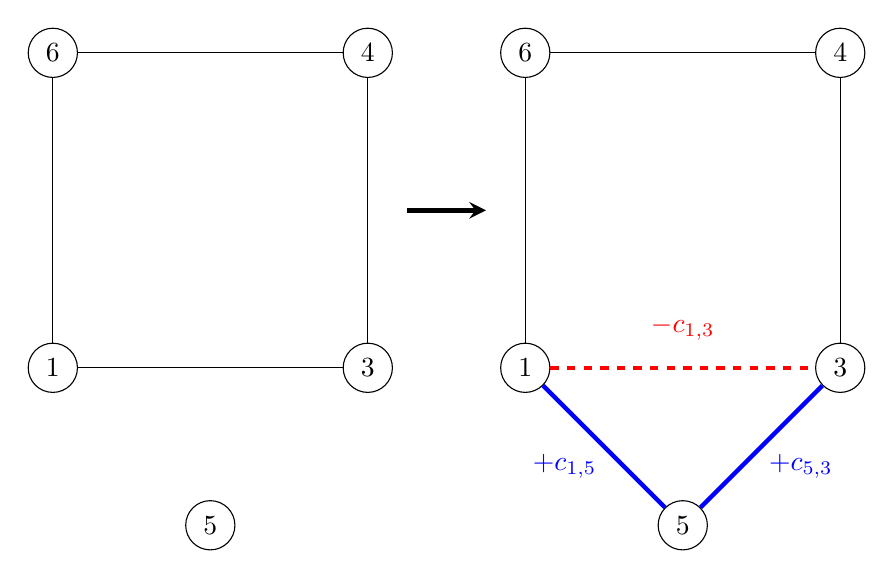
\begin{tikzpicture}
    \tikzstyle{vertex} = [circle, rounded corners, minimum width=0.5cm, minimum height=0.625cm,text centered, draw=black, fill=white]
    
    \node[vertex] (v1) at  (-2,-2) {1};
    \node[vertex] (v4) at  (2,2) {4};
    \node[vertex] (v6) at  (-2,2) {6};
    \node[vertex] (v3) at  (2,-2) {3};
    \node[vertex] (v5) at (0, -4) {5};
    
    \draw[-] (v1)--(v6);
    \draw[-] (v6)--(v4);
    \draw[-] (v4)--(v3);
    \draw[-] (v1)--(v3);
    
        
    \node[vertex] (v11) at  (4,-2) {1};
    \node[vertex] (v41) at  (8,2) {4};
    \node[vertex] (v61) at  (4,2) {6};
    \node[vertex] (v31) at  (8,-2) {3};
    \node[vertex] (v5) at (6, -4) {5};
    
    \draw[->,>=stealth, ultra thick] (2.5,0) -- (3.5,0);
    
    \draw[-] (v11)--(v61);
    \draw[-] (v61)--(v41);
    \draw[-] (v41)--(v31);
    \draw[dashed, color = red, ultra thick] (v11)-- node[yshift = 0.5cm]{\(-c_{1,3}\)}(v31);
    
    \draw[-, color = blue, ultra thick] (v11)-- node[xshift = -0.5cm, yshift = -0.25cm]{\(+c_{1,5}\)}(v5);
    \draw[-, color = blue, ultra thick] (v31)--node[xshift = 0.5cm, yshift = -0.25cm]{\(+c_{5,3}\)}(v5);
    
    \end{tikzpicture} 
    \caption{Inserção de um novo nó.}
    \label{fig:insercaoMaisBarata}
\end{figure}

É fácil perceber que escolher o vértice \(k\) e a aresta \(\{i,j\}\) de forma a minimizar \(\Delta\) significa diminuir o prejuízo no valor objetivo após a inserção. No entanto, escolher sempre o par \((k, \{i,j\})\) que minimiza \(\Delta\) pode ``viciar'' o método, levando-o sempre a soluções parecidas, o que pode dificultar as buscas locais. Portanto, convém introduzir um pouco de aleatoriedade na escolha do par. Baseando-se nessas ideias, pode-se enumerar as etapas do método Construção() como segue.

\begin{enumerate}
    \item Construir uma solução parcial \(s'\) de forma aleatória; \label{insercaomaisbaratainicio}
    \item \(V' \leftarrow \) vértices de \(s'\) e \(CL \leftarrow V \setminus V'\); 
    \item Computar os pares \((k, \{i,j\})\) para todo \(k \in CL\), \(\{i,j\} \in s'\) e armazená-los em uma lista \(\Omega\); \label{insercaomaisbarataloop}
    \item Ordenar os pares em \(\Omega\) em ordem crescente de \(\Delta\);
    \item \(\alpha \leftarrow\) número aleatório no intervalo \([0,1]\);
    \item Selecionar aleatoriamente um dos \(\lfloor \alpha \times |\Omega| \rfloor \) primeiros pares em \(\Omega\);
    \item Sendo \((k, \{i,j\})\) o par escolhido, retirar a aresta \(\{i,j\}\) de \(s'\) e inserir o vértice \(k\) entre $i$ e $j$;
    \item Remover \(k\) da lista de candidatos \(CL\);
    \item Se \(CL\) estiver vazio, retornar \(s'\). Senão, voltar para o passo \ref{insercaomaisbarataloop}.
\end{enumerate}

É suficiente construir o \textit{subtour} inicial do passo \ref{insercaomaisbaratainicio} com 3 vértices. Para isso, pode-se iniciar \(s'\) sempre como \texttt{s' = \{1, 1\}} e inserir 3 vértices de forma aleatória. Assim, o \textit{subtour} inicial da  Figura \ref{fig:insercaoMaisBarata}, por exemplo, seria \texttt{s' = \{1,6,4,3,1\}}.

Um exemplo de implementação do procedimento Construção() pode ser visto a seguir:

%\begin{lstlisting}[style=cplusplusListStyle, caption={Procedimento Construção().}, label={lst:construction}]
\begin{lstlisting}[style=cplusplusListStyle]
struct InsertionInfo
{
	int noInserido; // no k a ser inserido
	int arestaRemovida; // aresta {i,j} na qual o no k sera inserido
	double custo; // delta ao inserir k na aresta {i,j}
};
    
std::vector<InsertionInfo> calcularCustoInsercao(Solution& s, std::vector<int>& CL)
{
	std::vector<InsertionInfo> custoInsercao = std::vector<InsertionInfo> custoInsercao((s.size() - 1) * CL.size());
	int l = 0;	
	for(int a = 0; a < s.sequence.size() - 1; a++) {
		int i = s.sequence[a];
		int j = s.sequence[a + 1];
		for (auto k : CL) {
			custoInsercao[l].custo = c[i][k] + c[j][k] - c[i][j];
			custoInsercao[l].noInserido = k;
			custoInsercao[l].arestaRemovida = a;
			l++;
		}
	}
	return custoInsercao;
}

Solution Construcao()
{
	Solution s;
	s.sequence = escolher3NosAleatorios();
	std::vector<int> CL = nosRestantes();
	/* Ex: V = {1,2,3,4,5,6,7,8,9,10}
		 s.sequence = {1,2,9,5,1} 
		 CL = {3,4,6,7,8,10} */
	while(!CL.empty()) {
		std::vector<InsertionInfo> custoInsercao = calcularCustoInsercao(s, CL);
		ordenarEmOrdemCrescente(custoInsercao);
		double alpha = (double) rand() / RAND_MAX;
		int selecionado = rand() % ((int) ceil(alpha * custoInsercao.size()));
		inserirNaSolucao(s, custoInsercao[selecionado].k);
	}

    return s;
}
\end{lstlisting}

No exemplo, armazena-se as informações de cada par \((k, \{i,j\})\) em uma estrutura do tipo \texttt{InsertionInfo}. Os custos de inserção de cada par \((k, \{i,j\})\) são calculados pela função \texttt{calcularCustoInsercao()}, que é chamada na função \texttt{Construcao()} até que $CL$ esteja vazio.


\section{BuscaLocal()}
A etapa de busca local possui como objetivo melhorar a solução corrente no decorrer da execução do algoritmo. O procedimento é feito modificando-se as soluções e avaliando o impacto das modificações na função objetivo. Antes de descrever o procedimento BuscaLocal(), alguns conceitos são apresentados nas subseções que seguem.

\subsection{Movimentos}
Seja \(s\) uma solução viável qualquer para um problema de otimização, e \(m\) uma operação que altera \(s\) de alguma maneira. Diz-se que \(m\) é um ``movimento'', e que \(s' =  s \oplus m \) é  uma nova solução, obtida após executá-lo. Há varios tipos de movimentos possíveis, que dependem, por sua vez, do problema de otimização em questão. Um exemplo de movimento para o TSP é trocar as posições de dois vértices na sequência.

\subsection{Estruturas de vizinhança}
Sejam \(s\) uma solução qualquer, e \(M_k\) um conjunto de movimentos estruturalmente parecidos. O conjunto \(\mathcal{N}_k (s)\) contém todas as posíveis soluções que se poderia obter executando em \(s\) os movimentos do conjunto \(M_k\). Já que as soluções \(s\) e \(s' \in \mathcal{N}_k(s)\) diferem em apenas um movimento, diz-se que elas são ``vizinhas''. Por esse motivo, \(\mathcal{N}_k\) é considerado uma ``estrutura de vizinhança''. 

Para compreender melhor o conceito, consulte a Figura \ref{fig:exemploEstruturaVizinhanca}. Na figura, todas as combinações possíveis de movimentos da estrutura de vizinhança \textsc{Swap}, que envolve trocar a posição de dois vértices quaisquer na sequência, foram listadas para a solução \[s = (1, 3, 5, 2, 4, 6, 1).\]
 % \(\mathcal{N}_k (s) = \{s': s' = s \oplus m, m \in M_k \}\)

\begin{figure}
    \centering
    \scalebox{0.8}{
    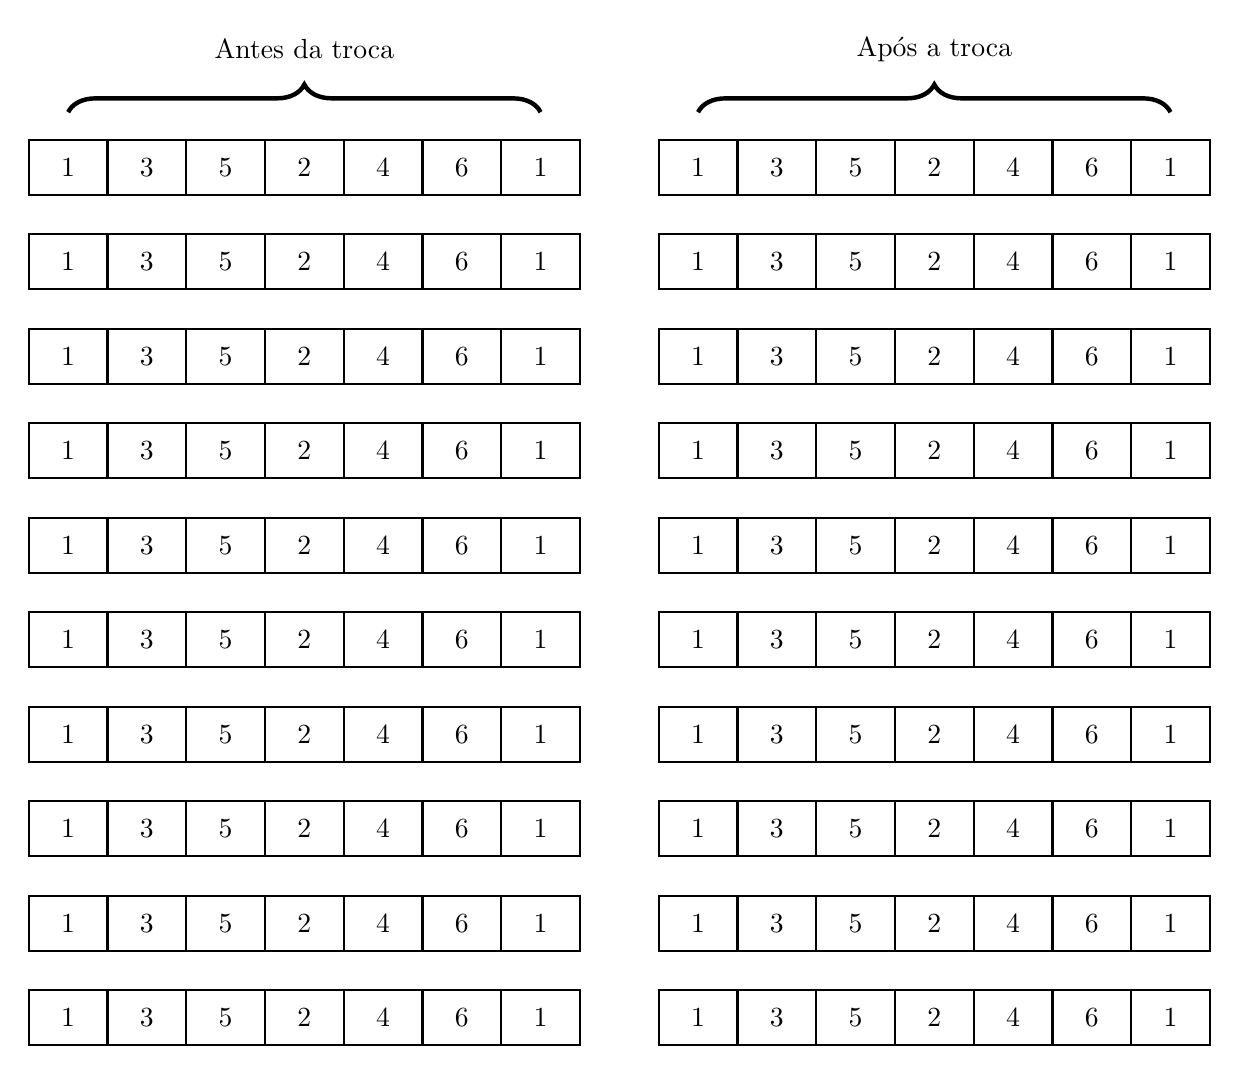
\begin{tikzpicture}
    

    
      \tikzstyle{vertexBlue} = [rectangle, draw=black, fill=white!30!, minimum height = 0.7cm, minimum width = 1cm, thick];
      \tikzstyle{vertexRed} = [rectangle, draw=black, fill=blue!30!, minimum height = 0.7cm, minimum width = 1cm, thick];
      \def\vertexArrayB{3,5,2,4,6};
      \def\n{6}
 %   \node[vertexBlue] at (0,1) {1};
 %   \foreach [count = \x] \i in \vertexArrayB
 %   {
%        \node[vertexBlue] at (\x,1) {\i};
   % }
    
  %  \node[vertexBlue] at (\n,1) {1};
    
    %%\draw [decorate,decoration={brace,amplitude=5pt,mirror,raise=4ex}, ultra thick]

        \draw [decorate,decoration={brace,amplitude=10pt}, ultra thick]
  (-4,-2) -- (-4+\n,-2) node[midway,yshift=0.8cm]{Antes da troca};
      
        \draw [decorate,decoration={brace,amplitude=10pt}, ultra thick]
  (4,-2) -- (4+\n,-2) node[midway,yshift=0.8cm]{Após a troca};
      
     \edef\mya{0}
      
      \foreach [count = \x from 1] \i in \vertexArrayB
      {
        \foreach [count = \y from 1] \j in \vertexArrayB
        {

            \ifnum \y > \x
            
            \pgfmathparse{\mya+1.5}
            \xdef\mya{\pgfmathresult}
            
            \node[vertexBlue] at (-4,-0.8*\mya -1.5) {\(1\)};

            \foreach [count = \z] \k in \vertexArrayB
            {
                \ifthenelse{\z = \x \OR \z = \y}{
                    \node[vertexRed] at (\z-4,-0.8*\mya - 1.5) {\(\k\)};
                }
                {
                    \node[vertexBlue] at (\z-4,-0.8*\mya - 1.5) {\(\k\)};
                }
            }
            
            \node[vertexBlue] at (-4+\n,-0.8*\mya -1.5) {\(1\)};

            \fi
            

        }
      }
      
       \edef\mya{0}
      
      \foreach [count = \x from 1] \i in \vertexArrayB
      {
        \foreach [count = \y from 1] \j in \vertexArrayB
        {

            \ifnum \y > \x
            
            \pgfmathparse{\mya+1.5}
            \xdef\mya{\pgfmathresult}
            
            \node[vertexBlue] at (0+4,-0.8*\mya -1.5) {\(1\)};

            \foreach [count = \z] \k in \vertexArrayB
            {
                \ifnum \z = \x
                    \node[vertexRed] at (4+\z,-0.8*\mya - 1.5) {\(\j\)};
                \fi
                
                \ifnum \z = \y
                    \node[vertexRed] at (4+\z,-0.8*\mya - 1.5) {\(\i\)};
                \fi
            
                \ifthenelse{\z = \x \OR \z = \y}{
                }
                {
                    \node[vertexBlue] at (4+\z,-0.8*\mya - 1.5) {\(\k\)};
                }
            }
            
            \node[vertexBlue] at (4+\n,-0.8*\mya -1.5) {\(1\)};

            \fi
            

        }
      }
      
     
    \end{tikzpicture}}
    \caption{Exemplo da estrutura de vizinhança \(swap\).}
    \label{fig:exemploEstruturaVizinhanca}
\end{figure}


\subsection{\textit{Best Improvement}}
Dada uma solução \(s\) e uma estrutura de vizinhança \(\mathcal{N}_k\), o método do melhor aprimoramento (\textit{best improvement}) visa encontrar o vizinho de $s$ com o menor custo possível. Em outras palavras, deseja-se encontrar o ``melhor vizinho'' de \(s\) considerando-se a estrutura de vizinhança \(\mathcal{N}_k\). Se \(f(s^*) < f(s)\), diz-se que houve uma melhora, e convém substituir \(s\) por \(s^*\). O trecho de código a seguir mostra como utilizar o método \textit{best improvement} para explorar toda a estrutura de vizinhança \(swap\):

%\begin{lstlisting}[style=cplusplusListStyle, caption={Função que determina o melhor vizinho de $s$.}, label={lst:bestImprovSwap}]
\begin{lstlisting}[style=cplusplusListStyle]
bool bestImprovementSwap(Solution *s)
{
	double bestDelta = 0;
	int best_i, best_j;
	for(int i = 1; i < s->sequence.size() - 1; i++)
	{
	    int vi = s->sequence[i];
	    int vi_next = s->sequence[i + 1];
	    int vi_prev = s->sequence[i - 1];
		for(int j = i + 1; j < s.sequence.size() - 1; j++)
		{
    	    int vj = s->sequence[j];
	        int vj_next = s->sequence[j + 1];
	        int vj_prev = s->sequence[j - 1];
	        double delta = -c[vi_prev][vi] -c[vi][vi_next] + c[vi_prev][vj] 
			               + c[vj][vi_next] - c[vj_prev][vj] - c[vj][vj_next] 
			               + c[vj_prev][vi] + c[vi][vj_next];
			               
				if (delta < bestDelta)
				{
					bestDelta = delta;
					best_i = i;
					best_j = j;
				}
		}
	}
            
	if(bestDelta < 0)
	{
		std::swap(s->sequence[best_i], s->sequence[best_j]);
		s->cost = s->cost + bestDelta;
		return true;
	}
	return false;
}
\end{lstlisting}

No código , enumera-se todos os movimentos de troca entre dois nós possíveis, e o impacto de cada movimento na função objetivo é avaliado nas linhas 15--17. Note que não é necessário recalcular o custo da solução do zero, pois o custo de uma troca pode ser calculado com uma simples fórmula desde que as arestas a serem removidas e inseridas sejam conhecidas\footnote{Levar isso em consideração é crucial para o bom desempenho do algoritmo.}.

\iffalse

Observe que, para cada par \(i\) e \(j\), \(\Delta\) poderia ser obtido fazendo-se \(\Delta \gets f(s\oplus \text{troca}(s_i,s_j)) - f(s)\). Porém, computar os custos \(f(s\oplus \text{troca}(s_i,s_j))\) e \(f(s)\) requer \(n\) operações de soma, ao passo que subtrair os custos das arestas removidas e adicionar os custos das arestas inseridas após a troca, como no Algoritmo \ref{alg:swapBestImprovement}, requer apenas uma única ``conta''. Isso tem um grande impacto no tempo de execução do algoritmo\footnote{Para visualizar isso, considere uma instância com 300 cidades. Computar \(f(s)\) ao avaliar cada possível movimento exigiria executar sempre 300 operações de soma. Computar o valor de \(\Delta\) como no Algoritmo \ref{alg:swapBestImprovement}, no entanto, exigiria sempre o mesmo número de operações, independentemente do tamanho da instância.}.

\begin{algorithm}
\DontPrintSemicolon
\KwIn{Sequência $s$ e número de vértices $n$}
%\KwOut{Sentence instances with cost-vectors for training $S_{i,c_i}$}
\tcp{Exemplo: s = \{1,5,4,3,6,2,1\}, n = 6}
\tcp{\(s_1\) = 1, \(s_2\) = 5, \(s_3\) = 4, ...}
\SetKwBlock{Begin}{função}{end função}
\Begin($\text{BestImprovementSwap} {(} s,n {)}$)
{
    $\Delta^* \gets 0$\; \label{algBestSwapIniciaDelta}
  \ForAll{$i = 2,\dots,n$} 
  {
    $\Delta_1 \gets -c_{s_i s_{i-1}} - c_{s_i s_{i+1}}$ \;
    \ForAll{$j = i + 1, \dots, n$}
    {
        \tcp{Caso especial: vértices adjacentes na sequência}
        \uIf{$j = i + 1$} 
        {
             $\Delta = -c_{s_i s_{i-1}} -c_{s_j s_{j+1}} + c_{s_{i-1} s_{j}} + c_{s_{j+1} s_i}$\;
            \lIf{$\Delta < \Delta^*$}
            {
                $i^*, j^*, \Delta^* \gets i,j,\Delta$ 
            }
        continue
        }
        \tcp{Vértices não adjacentes na sequência}
        \Else{
        $\Delta_2 \gets c_{s_j s_{i-1}} + c_{s_j s_{i+1}} - c_{s_j s_{j-1}} - c_{s_j s_{j+1}}+ c_{s_i s_{j-1}} + c_{s_i s_{j+1}}$  \;
        $\Delta = \Delta_1 + \Delta_2$\;
        \lIf{$\Delta < \Delta^*$}
        {
            $i^*, j^*, \Delta^* \gets i,j,\Delta$ 
        }
      %  \lElse
       % {continue}
       }
    }
   
  }\label{endfor}
  \lIf{$\Delta^* < 0$}
  {
    \(s \gets s \oplus \text{troca}(s_{i^*}, s_{j^*}), f(s) \gets f(s) + \Delta\)
  }
}
\caption{Algoritmo \textit{Best Improvement} para a estrutura de vizinhança \(swap\).}\label{alg:swapBestImprovement}
\end{algorithm}
\fi

\subsection{Estruturas de vizinhaça utilizadas}

As estruturas de vizinhança que devem ser utilizadas são descritas como segue.

\begin{itemize}
    \item \textsc{Swap} --- \(\mathcal{N}_1\): Troca a posição de dois vértices na sequência;
    \item \textsc{2-opt} --- \(N_2\): Duas arestas não adjacentes da solução são removidas e o segmento entre elas é reinserido de maneira invertida, adicionando-se duas novas arestas para reconstruir a solução.
    \item \textsc{Reinsertion} --- \(\mathcal{N}_3\): Um único vértice é retirado de sua posição e inserido em outra;
     \item \textsc{Or-opt-2} --- \(\mathcal{N}_4\): Um bloco composto por dois vértices adjacentes é retirado de sua posição e inserido em outra;
     \item \textsc{Or-opt-3} --- \(\mathcal{N}_5\): Um bloco composto por três vértices adjacentes é retirado de sua posição e inserido em outra;
\end{itemize}

A Figura \ref{fig:estruturasVizinhancaExemplos} apresenta exemplos de movimentos de cada uma das estruturas aplicados em uma solução com 10 vértices.

\begin{figure}[htpb!]
    \centering
        \subfloat[Solução original]{

        \centering
        \scalebox{0.8}{
        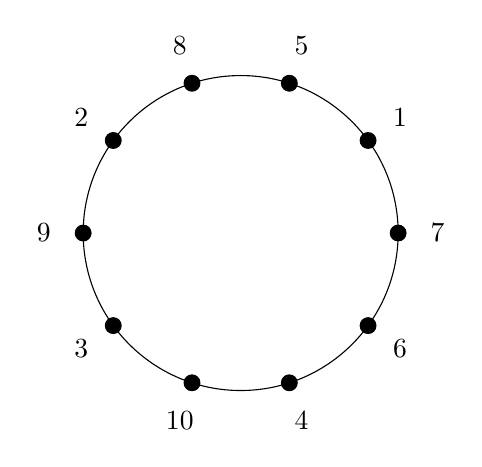
\begin{tikzpicture}
        \tikzstyle{arrow} = [->, >=latex]
        \tikzstyle{arrowblue} = [->,>=latex, color=red]
          
          \def\margin{2}
          
          \foreach [count = \x] \n in {1,5,8,2,9,3,10,4,6,7}
          {
          \node[circle, draw=black, fill=black, inner sep=0pt, minimum size = 0.2cm] (a\n) at ({(360*\x/(10))}:2) {};
           \node at ({(360*\x/(10))}:2.5) {\(\n\)};
          }
          
          \draw[-] (0:2) arc (0:360:2);
         
        \end{tikzpicture}
        \label{fig:exemploEstruturaOriginal}}}
        \hspace{0.5cm}
        \subfloat[\textsc{{Swap}}]{
        \centering
        \scalebox{0.8}{
          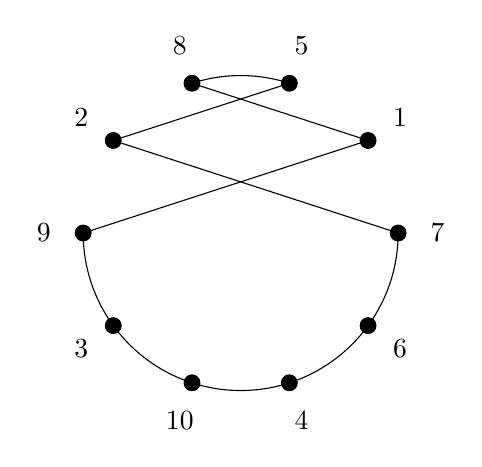
\begin{tikzpicture}
        \tikzstyle{arrow} = [->, >=latex]
        \tikzstyle{arrowblue} = [->,>=latex, color=red]
          
          \def\margin{2}
          
          \foreach [count = \x] \n in {1,5,8,2,9,3,10,4,6,7}
          {
          \node[circle, draw=black, fill=black, inner sep=0pt, minimum size = 0.2cm] (a\n) at ({(360*\x/(10))}:2) {};
           \node at ({(360*\x/(10))}:2.5) {\(\n\)};
          }
          
          \draw[-] (72:2) arc (72:72+36:2);
          \draw[-] (180:2) arc (180:360:2);
          \draw[-] (a7) to (a2);
          \draw[-] (a2) to (a5);
          \draw[-] (a8) to (a1);
          \draw[-] (a1) to (a9);
         
        \end{tikzpicture}
        \label{fig:exemploEstruturaSwap}}}
    \hspace{0.5cm}
    	\subfloat[\textsc{2-opt}.]{
        \centering
        \scalebox{0.8}{
          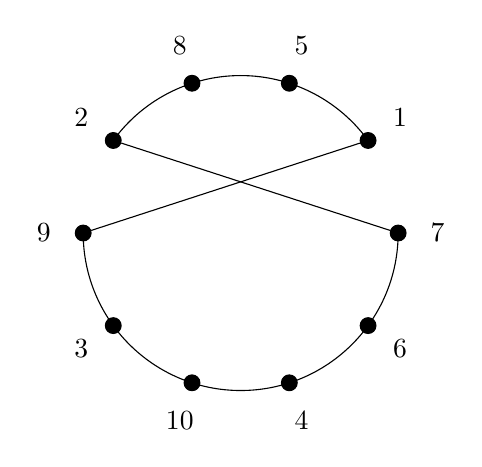
\begin{tikzpicture}
        \tikzstyle{arrow} = [->, >=latex]
        \tikzstyle{arrowblue} = [->,>=latex, color=red]
          
          \def\margin{2}
          
          \foreach [count = \x] \n in {1,5,8,2,9,3,10,4,6,7}
          {
          \node[circle, draw=black, fill=black, inner sep=0pt, minimum size = 0.2cm] (a\n) at ({(360*\x/(10))}:2) {};
           \node at ({(360*\x/(10))}:2.5) {\(\n\)};
          }
          
          \draw[-] (36:2) arc (36:4*36:2);
          \draw[-] (180:2) arc (180:360:2);
          \draw[-] (a1) to (a9);
          \draw[-] (a2) to (a7);
         
        \end{tikzpicture}
        \label{fig:exemploEstrutura2Opt}}}
    \hspace{0.5cm}
    \subfloat[\textsc{Reinsertion}.]{
        \centering
        \scalebox{0.8}{
          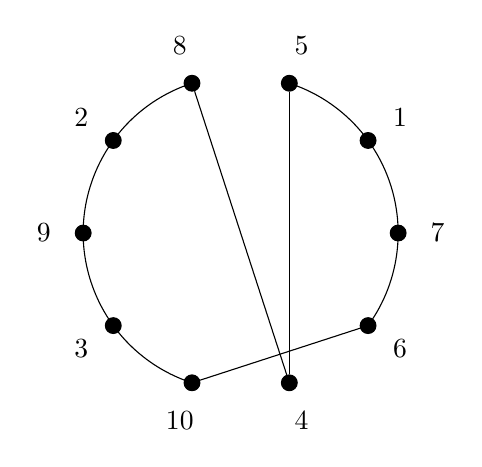
\begin{tikzpicture}
        \tikzstyle{arrow} = [->, >=latex]
        \tikzstyle{arrowblue} = [->,>=latex, color=red]
          
          \def\margin{2}
          
          \foreach [count = \x] \n in {1,5,8,2,9,3,10,4,6,7}
          {
          \node[circle, draw=black, fill=black, inner sep=0pt, minimum size = 0.2cm] (a\n) at ({(360*\x/(10))}:2) {};
           \node at ({(360*\x/(10))}:2.5) {\(\n\)};
          }
          
          \draw[-] (-36:2) arc (-36:2*36:2);
          \draw[-] (3*36:2) arc (3*36:7*36:2);
          \draw[-] (a4) to (a5);
          \draw[-] (a4) to (a8);
          \draw[-] (a10) to (a6);
        \end{tikzpicture}
        \label{fig:exemploEstruturaReinsertion}}}
    \hspace{0.5cm}
    	\subfloat[\textsc{Or-opt-2}]{
        \centering
        \scalebox{0.8}{
          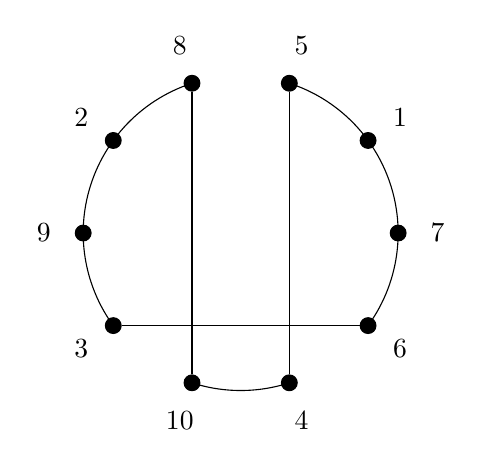
\begin{tikzpicture}
        \tikzstyle{arrow} = [->, >=latex]
        \tikzstyle{arrowblue} = [->,>=latex, color=red]
          
          \def\margin{2}
          
          \foreach [count = \x] \n in {1,5,8,2,9,3,10,4,6,7}
          {
          \node[circle, draw=black, fill=black, inner sep=0pt, minimum size = 0.2cm] (a\n) at ({(360*\x/(10))}:2) {};
           \node at ({(360*\x/(10))}:2.5) {\(\n\)};
          }
          
          \draw[-] (-36:2) arc (-36:2*36:2);
          \draw[-] (3*36:2) arc (3*36:6*36:2);
          \draw[-] (7*36:2) arc (7*36:8*36:2);
          
          \draw[-] (a4) to (a5);
          \draw[-] (a3) to (a6);
          \draw[-] (a10) to (a8);
        \end{tikzpicture}
        \label{fig:exemploEstruturaOrOpt2}}}
    \hspace{0.5cm}
    	\subfloat[\textsc{Or-opt-3}]{
        \centering
        \scalebox{0.8}{
          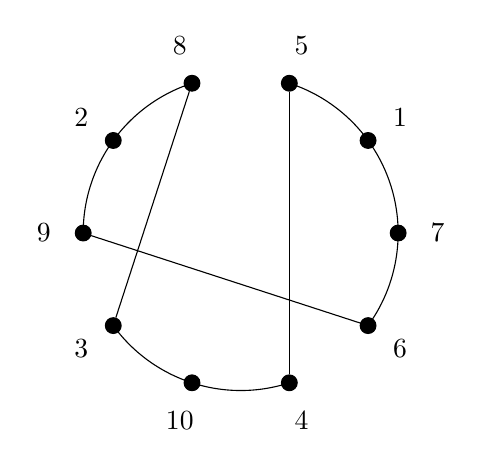
\begin{tikzpicture}
        \tikzstyle{arrow} = [->, >=latex]
        \tikzstyle{arrowblue} = [->,>=latex, color=red]
          
          \def\margin{2}
          
          \foreach [count = \x] \n in {1,5,8,2,9,3,10,4,6,7}
          {
          \node[circle, draw=black, fill=black, inner sep=0pt, minimum size = 0.2cm] (a\n) at ({(360*\x/(10))}:2) {};
           \node at ({(360*\x/(10))}:2.5) {\(\n\)};
          }
            \draw[-] (-36:2) arc (-36:2*36:2);
          \draw[-] (3*36:2) arc (3*36:5*36:2);
          \draw[-] (6*36:2) arc (6*36:8*36:2);
          
          \draw[-] (a4) to (a5);
          \draw[-] (a9) to (a6);
          \draw[-] (a3) to (a8);
        \end{tikzpicture}
        \label{fig:exemploEstruturaOrOpt3}}}

    
        \caption{Exemplos das estruturas de vizinhança.}


        \label{fig:estruturasVizinhancaExemplos}

\end{figure}


\subsection{RVND}
O procedimento BuscaLocal() consiste em uma implementação do método \textit{Random Variable Neighborhood Descent} (RVND) utilizando-se as estruturas de vizinhança mencionadas. A ideia do procedimento é utilizar o método \textit{best improvement} em diferentes estruturas de vizinhança (escolhidas de forma aleatória) enquanto houver melhora, eliminando estruturas de vizinhança que não provocaram melhoras. Isso pode ser visto no seguinte trecho de código:

%\begin{lstlisting}[style=cplusplusListStyle, caption = {Procedimento BuscaLocal() utilizando o método RVND.}, label = {lst:rvnd}]
\begin{lstlisting}[style=cplusplusListStyle]
void BuscaLocal(Solution *s)
{
  std::vector<int> NL = {1, 2, 3, 4, 5};
  bool improved = false;

  while (NL.empty() == false)
  {
    int n = rand() % NL.size();
    switch (NL[n])
    {
    case 1:
      improved = bestImprovementSwap(s);
      break;
    case 2:
      improved = bestImprovement2Opt(s);
      break;
    case 3:
      improved = bestImprovementOrOpt(s, 1); // Reinsertion
      break;
    case 4:
      improved = bestImprovementOrOpt(s, 2); // Or-opt2
      break;
    case 5:
      improved = bestImprovementOrOpt(s, 3); // Or-opt3
      break;
    }

    if (improved)
      NL = {1, 2, 3, 4, 5};
    else
      NL.erase(NL.begin() + n);
  }
}
\end{lstlisting}

\iffalse
\begin{enumerate}
    \item \(s' \gets s\);
    \item \(NL \gets \{\mathcal{N}_1,\dots,\mathcal{N}_5\}\); \label{buscalocalprimeiropasso}
    \item \(\mathcal{N}_\eta \gets \text{elemento aleatório de } NL\); \label{buscalocalsegundopasso}
    \item \(s_{temp} \gets s', \text{BestImprovement}(s', \mathcal{N}_\eta)\);
    \item Se \(f(s') < f(s_{temp})\), voltar para o passo \ref{buscalocalprimeiropasso};
    \item \(NL \gets NL \setminus \mathcal{N}_\eta\);
    \item Se \(NL = \emptyset\), retornar \(s'\). Caso contrário, voltar para o passo \ref{buscalocalsegundopasso}.
\end{enumerate}
\fi

No código, o procedimento BestImprovement() deve ser implementado para cada uma das 5 estruturas de vizinhança. A implementação de cada um dos procedimentos é semelhante ao exemplo mostrado anteriormente para a estrutura de vizinhança \textsc{Swap}.

 Já que as estruturas de vizinhança \textsc{Reinsertion}, \textsc{Or-opt-2} e \textsc{Or-opt-3} são muito parecidas, encoraja-se que sejam implementadas através de uma única função, que possui como um de seus parâmetros um número de 1 a 3, que representa o tamanho do bloco a ser movido.

\section{Perturbação()}

Uma solução é um ``ótimo local'' se ela não pode mais ser melhorada pelo procedimento BuscaLocal(). O objetivo do procedimento Perturbação() é modificar levemente soluções desse tipo. Embora uma solução obtida após uma perturbação aleatória seja quase sempre pior que a original, espera-se que ela possa ser melhorada através do procedimento BuscaLocal(), conforme ilustrado na Figura \ref{fig:buscaLocalExemplo}. 

Para facilitar a visualização, a função objetivo \(f(s)\) na Figura \ref{fig:buscaLocalExemplo} foi representada por meio de uma curva contínua, enquanto o eixo horizontal representa o espaço de soluções possíveis. As linhas tracejadas delimitam as soluções vizinhas que as buscas locais conseguem ``enxergar''. Ao realizar uma busca local nas vizinhanças de \(s_0\), obtém-se a solução \(s_1\), que é um ótimo local. A solução \(s_1\) é então perturbada, resultando em uma solução ligeiramente pior \(s_2\). Porém, ao realizar uma busca local nas vizinhanças de \(s_2\), obtém-se uma nova solução \(s_3\), que é o mínimo global da função. 


\begin{figure}
    \centering
    \scalebox{1.5}{
    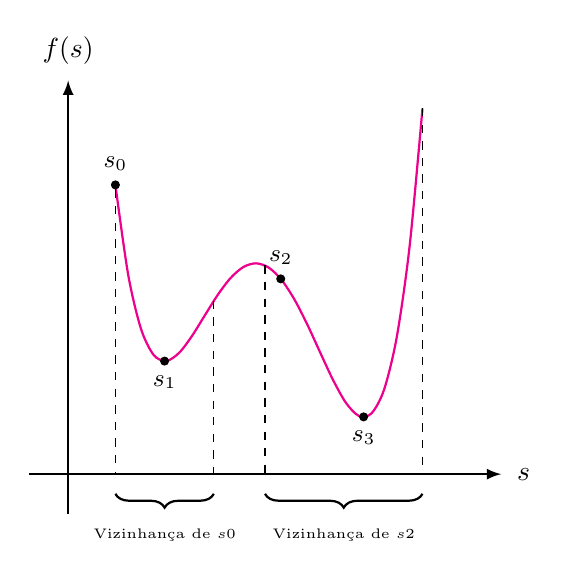
\begin{tikzpicture}
    \draw[->,>=latex, thick] (-1,0) -- (5,0) node[right = 2pt]{\(s\)};
    \draw[->, >=latex,thick] (-0.5,-0.5) -- (-0.5,5) node[above = 2pt]{\(f(s)\) };
    %\draw[thick] plot [smooth, tension = 0.5] coordinates{(0,4) (1,1)  (2,2) (3,0.3) (4,4)};
    
    \draw[domain=0.1:4, smooth, variable=\x, magenta,  thick] plot ({\x}, {6.166666/10*\x*\x*\x*\x - 4.816666666*\x*\x*\x +12.13333333*\x*\x - 10.933333333333*\x + 4.15 + 0.5});

    %  \draw[domain=0:4, smooth, variable=\x, magenta, thick] plot ({\x}, {24.7674*\x - 51.2235*\x*\x + 36.5566*\x*\x*\x - 10.6948*\x*\x*\x*\x + 1.09448*\x*\x*\x*\x*\x});




    \node[circle, draw=black,fill=black, inner sep = 0, minimum size = 0.1cm, label=above:{\small \(s_0\)}] (s0) at (0.1,3.67324) {};
    
    \node[circle, draw=black,fill=black, inner sep = 0, minimum size = 0.1cm, label=below:{\small \(s_1\)}] (s1) at (0.724347,0.935762 + 0.5) {};
    
    \node[circle, draw=black,fill=black, inner sep = 0, minimum size = 0.1cm, label=above:{\small \(s_2\)}] (s2) at (2.2,2.47992) {};
    
    \node[circle, draw=black,fill=black, inner sep = 0, minimum size = 0.1cm, label=below:{ \small \(s_3\)}] (s3) at (3.2522,0.22712 + 0.5) {};
    
   \draw[-, dashed] (s0) -- (0.1,0);
   \draw[-, dashed] (1.35,2.20046) -- (1.35,0);
   \draw[-, dashed] (2,2.65) -- (2,0);
   \draw[-, dashed] (4,4.64998) -- (4,0);

    \draw[decorate,decoration={brace,amplitude=5pt, mirror}, thick] (0.1, -0.25) -- (1.35,-0.25) node[midway, yshift = -15pt, font=\tiny]{{Vizinhança de \(s0\)}};
    \draw[decorate,decoration={brace,amplitude=5pt, mirror}, thick] (2, -0.25) -- (4,-0.25) node[midway, yshift = -15pt, font=\tiny]{{Vizinhança de \(s2\)}};
    
   %% \draw[->, >=latex, color = blue!50!, thick] plot [smooth, tension = 0.5]  coordinates{(0.95, 1.45) (1.55, 1.65) (2.1, 2.38) } node[yshift=0.8cm, xshift=-0.5cm] {};

   %% \draw[->, >=latex, color = orange!50!, thick] plot [smooth, tension = 0.5]  coordinates{(-0.2, 3.45) (0.0, 2) (0.55, 1.3) } node[yshift=0.8cm, xshift=-1.5cm] {};

 %%  \draw[->, >=latex, color = orange!50!, thick] plot [smooth, tension = 0.5]  coordinates{(2.2, 2.25) (2.4, 1.1) (3.05, 0.75) } node[yshift=0.8cm, xshift=-0.5cm] {};


    \end{tikzpicture} 
    }
    \caption{Visualização da busca local.}
    \label{fig:buscaLocalExemplo}
\end{figure}

Neste caso, o procedimento Perturbação() consiste na execução de um movimento chamado \textit{double bridge}. O movimento troca as posições de dois segmentos da sequência. As figuras \ref{fig:solAntesDB} e \ref{fig:solAposDB} ilustram um exemplo de uma solução antes e após esse movimento. 

Uma chamada ao procedimento Perturbação(\(s\)) deve executar os seguintes passos:

\begin{enumerate}
    \item \(s' \gets s\);
    \item Escolher aleatoriamente dois segmentos não sobrepostos de \(s'\) de tamanhos entre \(2\) e \(\lceil |V|/10 \rceil\);
    \item Trocar a posição dos segmentos em \(s'\);
    \item Retornar \(s'\).
\end{enumerate}



\begin{figure}[htpb!]
    \centering
	\subfloat[Solução antes da perturbação.]{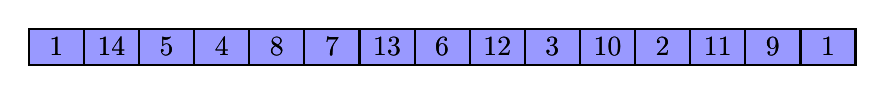
\begin{tikzpicture}
	\foreach[count = \i] \x in {1,14,5,4,8,7,13,6,12,3,10,2,11,9,1}{
		\ifthenelse{\i=3 \OR \i=4 \OR \i=10 \OR \i=11 \OR \i=12 \OR \i = 13}{
			\node[draw, thick, minimum width=0.7cm, fill=blue!40]  at (\i*0.7,0) {\x};		
		}
		{
			\node[draw, thick, minimum width=0.7cm]  at (\i*0.7,0) {\x};		
		}
	}
    \end{tikzpicture}\label{fig:solAntesDB}}
    \qquad
	\subfloat[Solução após a perturbação.]{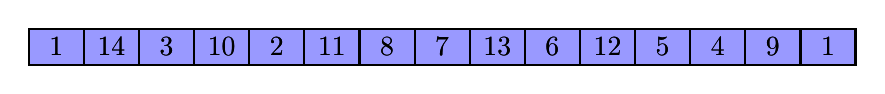
\begin{tikzpicture}
	\foreach[count = \i] \x in {1,14,3,10,2,11,8,7,13,6,12,5,4,9,1}{
		\ifthenelse{\i=3 \OR \i=4 \OR \i=5 \OR \i=6 \OR \i=12 \OR \i=13}{
			\node[draw, thick, minimum width=0.7cm, fill=blue!40]  at (\i*0.7,0) {\x};		
		}
		{
			\node[draw, thick, minimum width=0.7cm]  at (\i*0.7,0) {\x};		
		}
	}
    \end{tikzpicture}\label{fig:solAposDB}}


    \caption{Exemplo do movimento \textit{double bridge} em uma sequência.}
    \label{fig:exemploDoubleBridge}
\end{figure}



\iffalse
\begin{figure}[t]
    \centering
        \begin{subfigure}[b]{0.4\textwidth}
        \centering
        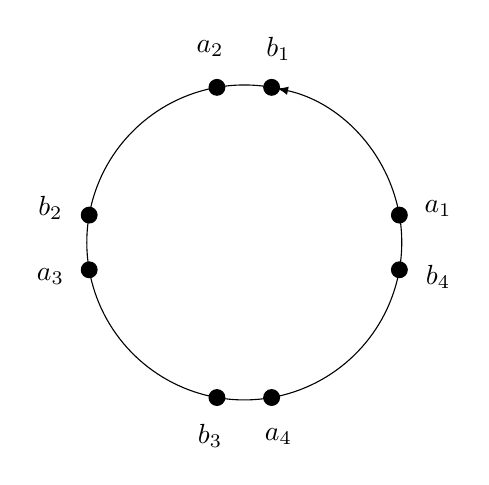
\begin{tikzpicture}
        \tikzstyle{arrow} = [->, >=latex]
        \tikzstyle{arrowblue} = [->,>=latex, color=red]
          
          \def\margin{2}
          
          \foreach [count = \x] \n in {0,...,3}
          {
          \node[circle, draw=black, fill=black, inner sep=0pt, minimum size = 0.2cm] (a\x) at ({(360*\n/(4)) + 10}:2) {};
          \node[circle, draw=black, fill=black, inner sep=0pt, minimum size = 0.2cm] (b\x) at ({(360*\n/(4)) - 10}:2) {};
           \node at ({(360*\n/(4)) + 10}:2.5) {\(a_\x\)};
           \node at ({(360*\n/(4)) + 80}:2.5) {\(b_\x\)};
          }
         
         \draw[arrow] (10:2) arc ({10}:{80-\margin}:2);
         \draw[-] (100:2) arc ({100}:{170-\margin}:2);
         \draw[-] (190:2) arc ({190}:{260-\margin}:2);
         \draw[-] (280:2) arc ({280}:{350-\margin}:2);
         
         \draw[-] (80:2) arc ({80}:{100-\margin}:2);
         \draw[-] (170:2) arc ({170}:{190-\margin}:2);
         \draw[-] (260:2) arc ({260}:{280-\margin}:2);
         \draw[-] (-10:2) arc ({-10}:{10-\margin}:2);
        \end{tikzpicture}
        \caption{Solução antes do \textit{double bridge}}
        \label{fig:antesDoubleBridge}
    \end{subfigure}
    \hspace{0.5cm}
    \begin{subfigure}[b]{0.4\textwidth}
        \centering
        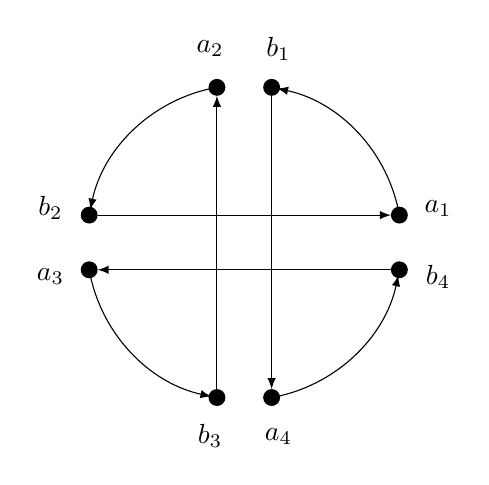
\begin{tikzpicture}
        \tikzstyle{arrow} = [->, >=latex]
        
        \def\margin{2}

         \foreach [count = \x] \n in {0,...,3}
          {
          \node[circle, draw=black, fill=black, inner sep=0pt, minimum size = 0.2cm] (a\x) at ({(360*\n/(4)) + 10}:2) {};
          \node[circle, draw=black, fill=black, inner sep=0pt, minimum size = 0.2cm] (b\x) at ({(360*\n/(4)) - 10}:2) {};
           \node at ({(360*\n/(4)) + 10}:2.5) {\(a_\x\)};
           \node at ({(360*\n/(4)) + 80}:2.5) {\(b_\x\)};
          }
          
         \draw[arrow] (10:2) arc ({10}:{80-\margin}:2);
         \draw[arrow] (100:2) arc ({100}:{170-\margin}:2);
         \draw[arrow] (190:2) arc ({190}:{260-\margin}:2);
         \draw[arrow] (280:2) arc ({280}:{350-\margin}:2);
         
         \draw[arrow] (b3) -- (a1);
         \draw[arrow] (b4) -- (a2);
         \draw[arrow] (b1) -- (a3);
         \draw[arrow] (b2) -- (a4);
        \end{tikzpicture}
        \caption{Solução após o \textit{double bridge}}
        \label{fig:aposDoubleBridge}
    \end{subfigure}
    
        \caption{Movimento \textit{double bridge}.}
        \label{fig:doubleBridge}

\end{figure}
\fi


\section{Parâmetros}
Os parâmetros \texttt{maxIter} e \texttt{maxIterIls} influenciam no desempenho no algoritmo tanto em termos de tempo, quanto na qualidade das soluções. Neste caso, os valores dos parâmetros devem ser inicializados da seguinte forma:
\begin{enumerate}
    \item \(\texttt{maxIter} \gets 50\);
    \item \(\texttt{maxIterILS} \gets \begin{cases}{|V|/2} \text{ se } |V| \geq 150 \\
            |V| \text{ senão}.
            \end{cases}\)
\end{enumerate}

\section{\textit{Benchmark}}

A Tabela \ref{tab:tabelaResultadosIlsTsp} apresenta os valores médios de custo e tempo (em segundos) de resolução de cada instância após 10 execuções do algoritmo em um Intel® Core™ i7-3770 3.40GHz.

\begin{table}[tp!]
\caption{Tempo e custo médios obtidos para cada instância.}
\label{tab:tabelaResultadosIlsTsp}
\centering
{
\setlength{\tabcolsep}{12pt}
\scriptsize
\centering
%\rowcolors{4}{black!7}{white}
\begin{tabular}{cccccc}
\toprule
\multirow{2.5}{*}{\textbf{Instância}} & \multicolumn{2}{c}{\textbf{Resultados}} & \multirow{2.5}{*}{\textbf{Instância}} & \multicolumn{2}{c}{\textbf{Resultados}} \\
\cmidrule{2-3}\cmidrule{5-6}
& \textbf{Tempo} & \textbf{Custo} & & \textbf{Tempo}   & \textbf{Custo} \\ 
%\cmidrule{2-3}\cmidrule{5-6}
\midrule
\texttt{a280}      &  96,623   & 2579    & \texttt{kroA150}   & 11,751  & 26524   \\
\texttt{ali535}    &  1525     & 202384  & \texttt{kroA200}   & 32,951  & 29368   \\
\texttt{att48}     &  0,3      & 10628   & \texttt{kroB100}   & 3,748   & 22141   \\
\texttt{att532}    &  1778,96  & 27731   & \texttt{kroB150}   & 10,634  & 26130   \\
\texttt{bayg29}    &  0,043    & 1610    & \texttt{kroB200}   & 35,53   & 29437,2 \\
\texttt{bays29}    &  0,05     & 2020    & \texttt{kroC100}   & 3,568   & 20749   \\
\texttt{berlin52}  &  0,374    & 7542    & \texttt{kroD100}   & 4,114   & 21294   \\
\texttt{bier127}   &  10,209   & 118282  & \texttt{kroE100}   & 3,745   & 22068   \\
\texttt{brazil58}  &  0,479    & 25395   & \texttt{lin105}    & 4,355   & 14379   \\
\texttt{brg180}    &  12,824   & 1950    & \texttt{lin318}    & 188,78  & 42045,7 \\
\texttt{burma14}   &  0,004    & 3323    & \texttt{linhp318}  & 187,536 & 42053,1 \\
\texttt{ch130}     &  10,91    & 6110    & \texttt{pcb442}    & 597,431 & 50876   \\
\texttt{ch150}     &  10,43    & 6528    & \texttt{pr107}     & 4,582   & 44303   \\
\texttt{d198}      &  33,639   & 15780   & \texttt{pr124}     & 7,021   & 59030   \\
\texttt{d493}      &  1132,48  & 35042   & \texttt{pr136}     & 13,632  & 96772   \\
\texttt{dantzig42} &  0,161    & 699     & \texttt{pr144}     & 10,479  & 58537   \\
\texttt{eil101}    &  4,436    & 629     & \texttt{pr152}     & 8,708   & 73682   \\
\texttt{eil51}     &  0,369    & 426     & \texttt{pr226}     & 45,27   & 80369   \\
\texttt{eil76}     &  1,549    & 538     & \texttt{pr264}     & 64,758  & 49135   \\
\texttt{fl417}     &  365,503  & 11861   & \texttt{pr299}     & 130,098 & 48194,8 \\
\texttt{fri26}     &  0,033    & 937     & \texttt{pr76}      & 1,366   & 108159  \\
\texttt{gil262}    &  82,271   & 2378,7  & \texttt{rat195}    & 28,046  & 2326,1  \\
\texttt{gr120}     &  9,065    & 6942    & \texttt{rat99}     & 4,115   & 1211    \\
\texttt{gr137}     &  11,348   & 69853   & \texttt{rd100}     & 3,983   & 7910    \\
\texttt{gr17}      &  0,008    & 2085    & \texttt{rd400}     & 498,288 & 15296,1 \\
\texttt{gr202}     &  37,105   & 40160,1 & \texttt{si175}     & 17,333  & 21407   \\
\texttt{gr21}      &  0,014    & 2707    & \texttt{si535}     & 758,534 & 48466,8 \\
\texttt{gr229}     &  61,498   & 134613  & \texttt{st70}      & 1,03    & 675     \\
\texttt{gr24}      &  0,028    & 1272    & \texttt{swiss42}   & 0,155   & 1273    \\
\texttt{gr431}     &  721,745  & 171530  & \texttt{ts225}     & 28,869  & 126643  \\
\texttt{gr48}      &  0,314    & 5046    & \texttt{tsp225}    & 45,368  & 3916    \\
\texttt{gr96}      &  3,475    & 55209   & \texttt{u159}      & 10,828  & 42080   \\
\texttt{hk48}      &  0,336    & 11461   & \texttt{ulysses16} & 0,008   & 6859    \\
\texttt{kroA100}   &  3,468    & 21282   & \texttt{ulysses22} & 0,019   & 7013    \\
\bottomrule
\end{tabular}
}
\end{table}
%%%%%%%%%%%%%%%%%%%%%%%%%%%%%%%%%%%%%%%%%%%%%%%%%%%%
\iffalse
\chapter*{COLOCAR EM ALGUM LUGAR}
{\color{red}EVITANDO O USO DE POO, REFERÊNCIAS, ETC. (A.K.A ``PROGRAMAÇÃO ORIENTADA A \textit{STRUCTS}'', OU ``DESORIENTAÇÃO A OBJETOS'')}

\begin{lstlisting}[label=exemploStructSolucao, caption=Representação das soluções, style=cplusplusListStyle]
typedef struct Solucao{
    vector<int> sequencia;
    double valorObj;
} Solucao;

\end{lstlisting}

\begin{lstlisting}[label=exemploInicializacaoInsercao, caption=Inicialização de soluções e inserção de vértices, style=cplusplusListStyle] 
// Exemplo de inicializacao 
Solucao s1 = {{1,6,3,2,5,4,1}, 902.0};

// Iterando pelos vertices da solucao 
void exibirSolucao(Solucao *s)
{
    for(int i = 0; i < s->sequencia.size() - 1; i++)
        std::cout << s->sequencia[i] << " -> ";
    std::cout << s->sequencia.back() << std::endl;
}

exibirSolucao(&s1);
// RESULTADO: "1 -> 6 -> 3 -> 2 -> 5 -> 4 -> 1" 

// Inicializando uma solucao vazia 
Solucao s2 = {{}, 0.0};
// Adicionando vertices na solucao 
s2.push_back(1);
s2.push_back(3);
s2.push_back(1);
exibirSolucao(&s2);
// RESULTADO: "1 -> 3 -> 1"
s2.insert(s2.begin() + 1, 4);
s2.insert(s2.end() - 1, 5);
s2.insert(s2.begin() + 2, 2);
exibirSolucao(&s2);
// RESULTADO: "1 -> 4 -> 2 -> 3 -> 5 -> 1"
\end{lstlisting}


\begin{lstlisting}[label=exemploCalculoValorObj, caption=Cálculo do valor objetivo, style=cplusplusListStyle]
void calcularValorObj(Solucao *s){
    s->valorObj = 0;
    for(int i = 0; i < s->sequencia.size() - 1; i++)
        s->valorObj += MatrizDistancia[s->sequencia[i]][s->sequencia[i+1]];
}
\end{lstlisting}





\begin{lstlisting}[style=cplusplusListStyle, caption=Cálculo de custo de inserção., label=exemploCalculoCustoInsercao]
typedef struct InfoInsercao
{
    int noInserido; // vertice k
    int arestaRemovida; // aresta {i,j}
    double custoInsercao; // impacto ao remover a aresta {i,j} e inserir o vertice k entre i e j
} InfoInsercao;
    
std::vector<InfoInsercao>();

for(int aresta = 0, idx = 0; aresta < s.size() - 1; aresta++, idx++)
{
    for (auto k : listaDeCandidatos)
    {
        int i = s->sequencia[idx];
        int j = s->sequencia[idx+1];
        InfoInsercao info;
        info.custo = MatrizDistancia[i][k] + MatrizDistancia[j][k] - MatrizDistancia[i][j];
        info.noInserido = k;
        info.arestaRemovida = aresta;
        custoInsercao.push(info);
    }
}
\end{lstlisting}

\begin{lstlisting}[style=cplusplusListStyle, caption=Estrutura de vizinhança \textbf{swap}., label=exemploBestImproveSwapCodigo]
void BestImprovementSwap(Solution *s, double **matrizAdj){
    double bestDelta = 0;
    int n = s.size();
    int best_i_idx, best_j_idx;
    double **c = matrizAdj;
    for (int idx_i = 1; idx_i < n - 1; idx_i++){
        int i = s->sequence[idx_i], next_i = s->sequence[idx_i+1], prev_i->sequence = s[idx_i-1];
        for (int idx_j = idx_i+1; idx_j < n - 1; idx_j++){
            int j = s->sequence[idx_j], next_j = s->sequence[idx_j+1], prev_j = s->sequence[idx_j-1];
            double delta;
            // Caso especial: vertices adjacentes
            if(j == next_i)
                delta = -c[i][prev_i] - c[j][next_j] + c[j][prev_i] + c[i][next_j];
            else
                delta = -c[i][prev_i] - c[i][next_i] - c[j][next_j] - c[j][prev_j] + c[j][prev_i] + c[j][next_i] + c[i][prev_j] + c[i][next_j];
            
            if (delta < bestDelta)
            {
                bestDelta = delta;
                best_i_idx = i;
                best_j_idx = j;
            }
        }
    }
    if (bestDelta < 0)
            std::swap(s->sequence[best_i_idx], s->sequence[best_j_idx]);
}
\end{lstlisting}
\fi
